You have to submit exactly one file, called \texttt{friend.cpp}. This file should implement the subprogram described above, using the following signatures. You also need to include a header file \texttt{friend.h} for C/C++ implementation.

\begin{center}
\renewcommand{\arraystretch}{1.5}
\begin{tabular}{|c|c|c|c|}
\hline
stage & host & protocol & friend relations added\\
\hline
1 &  0 & IAmYourFriend &  (1, 0) \\
\hline
2 & 0 & MyFriendsAreYourFriends & (2, 1) \\
\hline
3 & 1 & WeAreYourFriends & (3, 1), (3, 0), (3, 2)  \\
\hline
4 & 2 & MyFriendsAreYourFriends & (4, 1), (4, 3) \\
\hline
5 & 0 & IAmYourFriend & (5, 0) \\
\hline
\end{tabular}
\end{center}

Initially the network contains only person 0. The host of stage 1 (person 0) invites the new person 1 through the \texttt{IAmYourFriend} protocol, hence they become friends. The host of stage 2 (person 0 again) invites person 2 by \texttt{MyFriendsAreYourFriends}, which makes person 1 (the only friend of the host) the only friend of person 2. The host of stage 3 (person 1) adds person 3 through \texttt{WeAreYourFriends}, which makes person 3 a friend of person 1 (the host) and people 0 and 2 (the friends of the host). Stages 4 and 5 are also shown in the table above. The final network is shown in the following figure, in which the numbers inside the circles show the labels of people, and the numbers next to the circles show the survey confidence. The sample consisting of people 3 and 5 has totalsurvey confidence equal to $20 + 15 = 35$, which is the maximum possible total confidence.

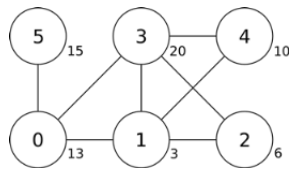
\includegraphics{1.png}